\documentclass[usenames,dvipsnames,svgnames,table,a4paper,openany,justified]{tufte-book}
\usepackage[utf8]{inputenc}
%\usepackage{draftwatermark}
\usepackage[T1]{fontenc}
\usepackage{geometry, graphicx}
\usepackage{amsmath}
\usepackage{caption}
\usepackage{subfig}
\usepackage{amssymb,amsfonts,textcomp}
\usepackage{polski}
\usepackage[english,polish]{babel}
\usepackage{color}
\usepackage{tcolorbox}
\tcbuselibrary{skins}
\usepackage{array}
\usepackage{supertabular}
\usepackage{hhline}
\usepackage{hyperref}
\usepackage{glossaries}
\usepackage{indentfirst}
\usepackage{import}
\hypersetup{colorlinks=true, linkcolor=blue, citecolor=blue, filecolor=blue, urlcolor=blue}
\usepackage{xcolor}
\graphicspath{ {skryptkierownik-img/} }
\definecolor{titlepagecolor}{cmyk}{0.7,.30,0,.40}
\definecolor{miejscekolor}{cmyk}{0,0,1,.10}
\definecolor{qgismaincolor}{cmyk}{70.53,18.84,100,3.7}
\definecolor{code-gray}{gray}{0.95}
%\SetWatermarkText{}
%\SetWatermarkScale{0.3}
%\SetWatermarkColor[rgb]{0.7,0.4,0.4}
\makeglossaries
\author{Tomasz Nycz (red.)}
\title{Kurs Kierownika Pociągu}
% For A4 paper
\geometry{
	left=18mm, % left margin
	textwidth=130mm, % main text block
	marginparsep=8mm, % gutter between main text block and margin notes
	marginparwidth=52mm % width of margin notes
}
\begin{document}
	\setlength{\parindent}{1cm} % Default is 15pt.
\begin{titlepage}
	\newgeometry{left=5cm} %defines the geometry for the titlepage
	\pagecolor{titlepagecolor}
	\noindent
	\color{white}
	\makebox[0pt][l]{\rule{1.3\textwidth}{1pt}}
	\par
	\noindent
	\textbf{\textsf{Materiały szkoleniowe}} \\
	\noindent 
	\textcolor{miejscekolor}{\textsf{Praca zbiorowa pod troskliwą opieką instruktorów}}\\
	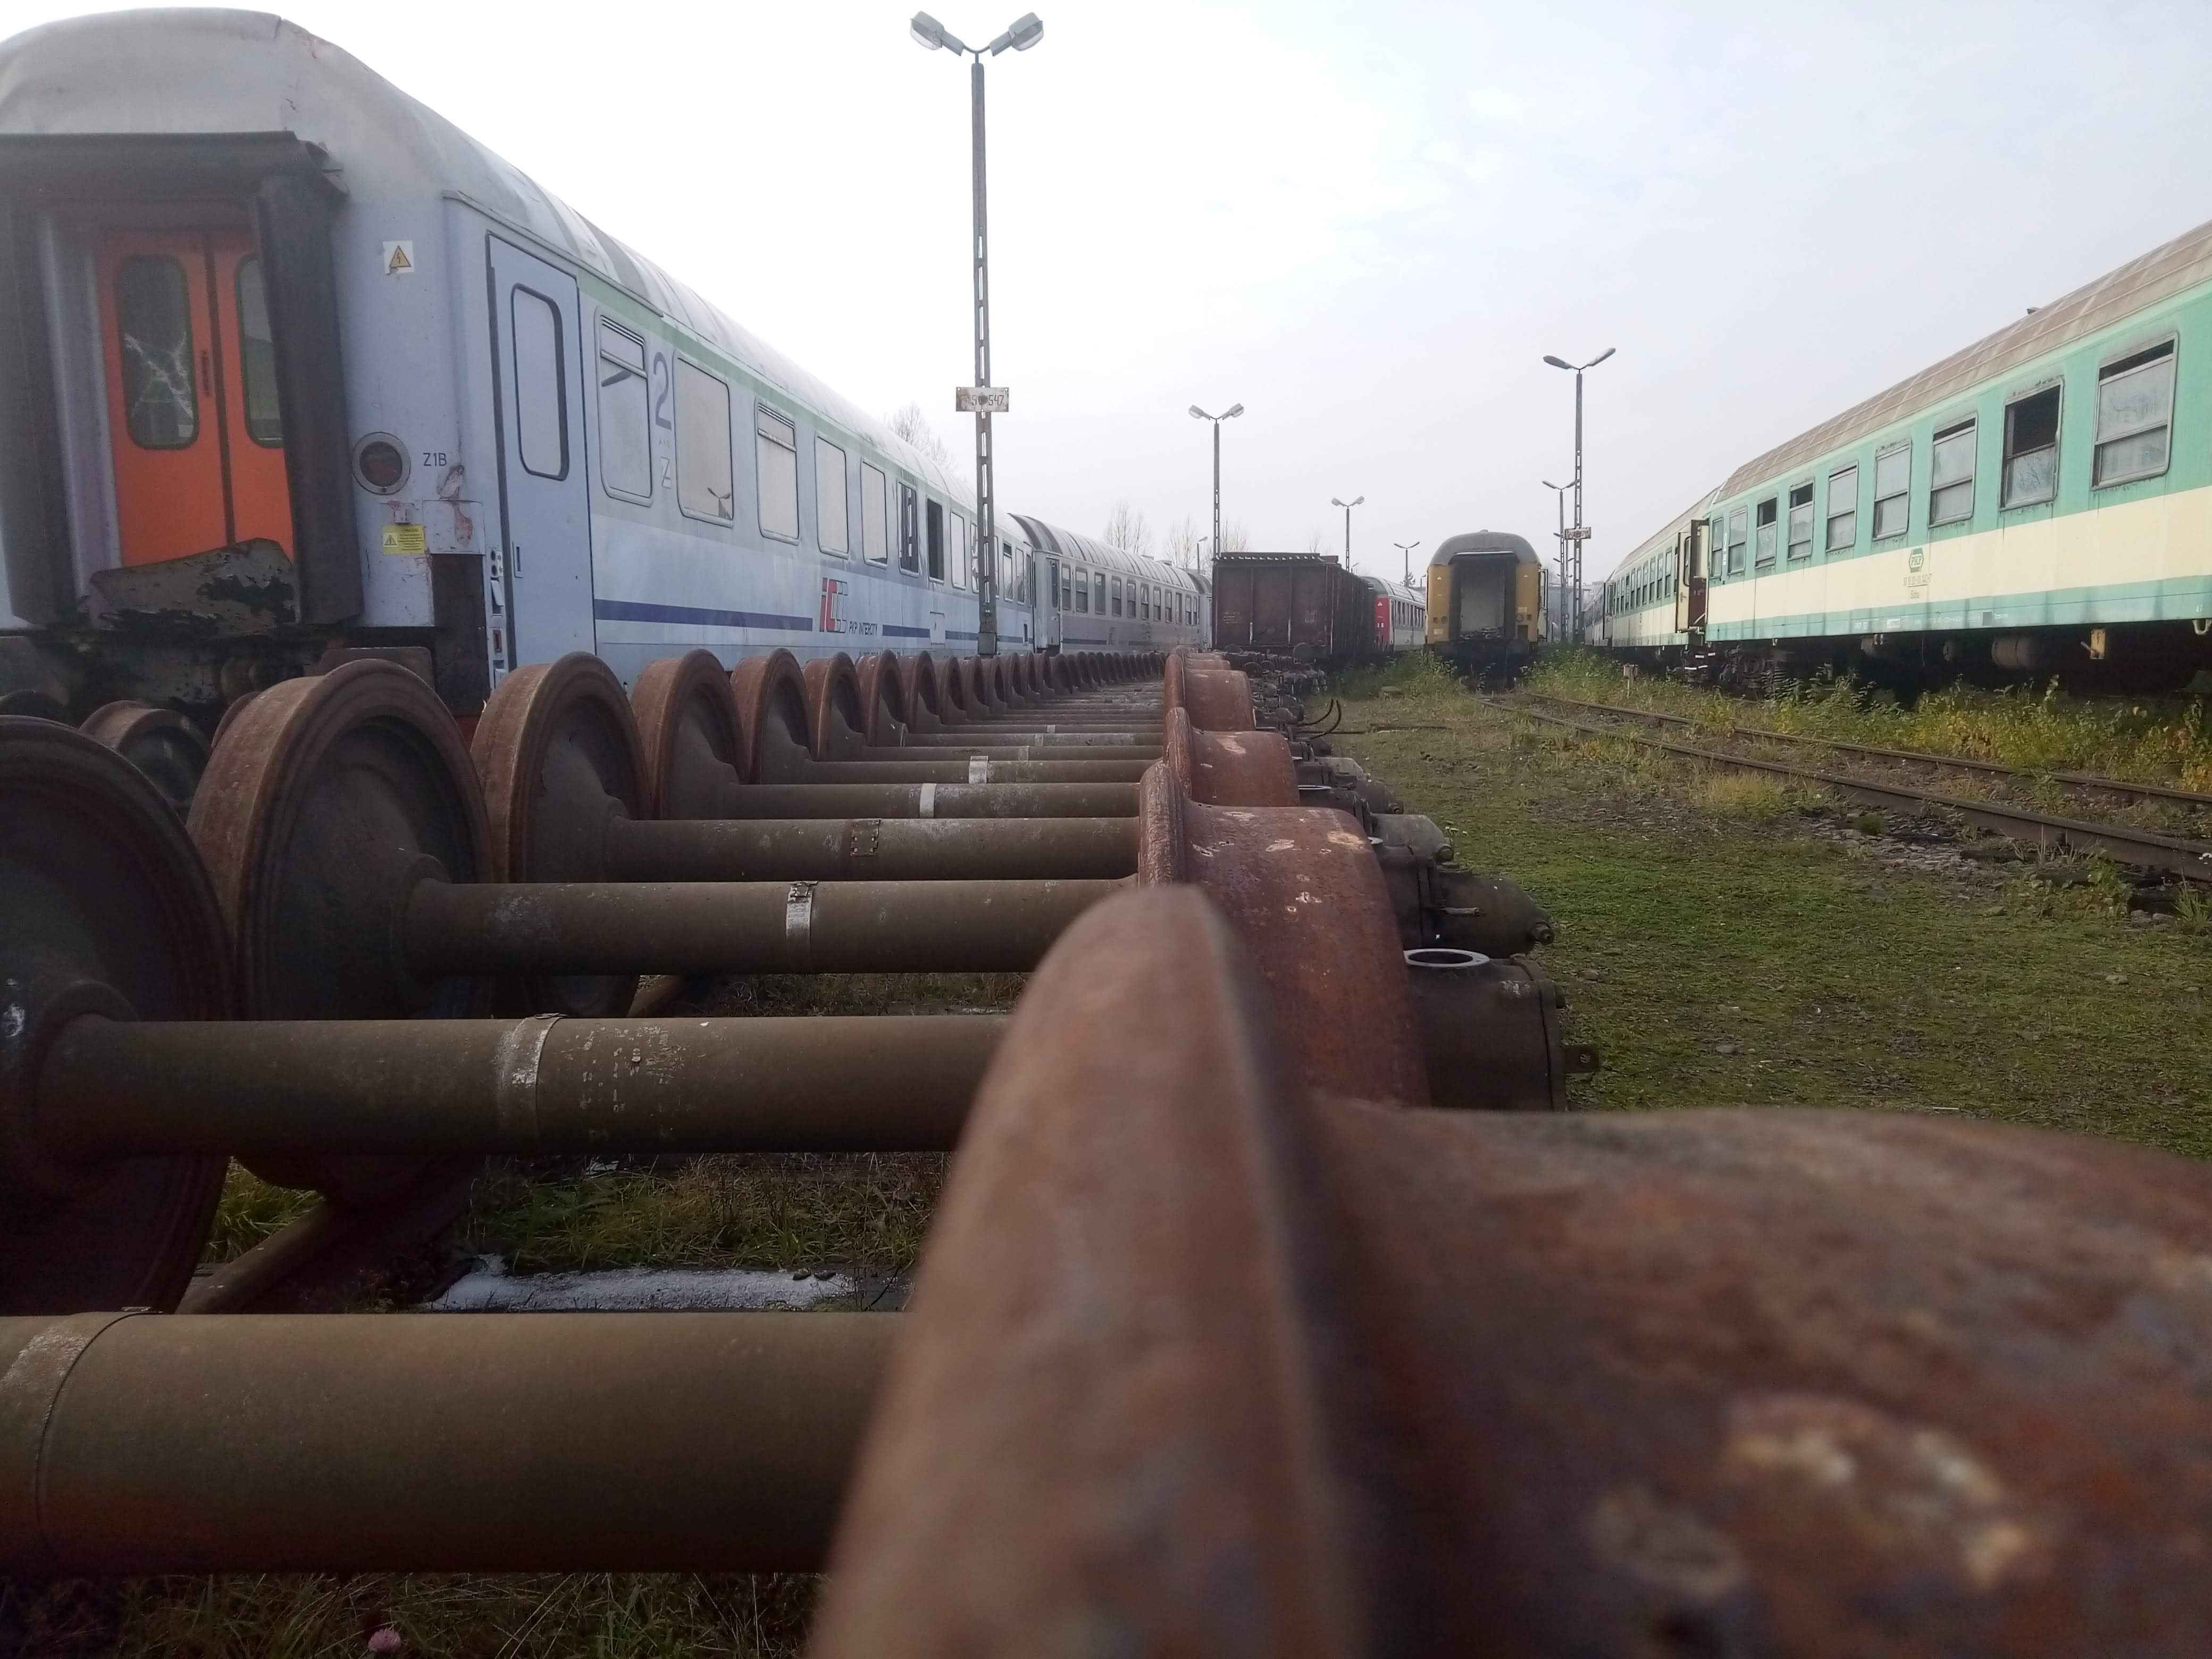
\includegraphics[width=16cm]{kolka.jpg}
	\vfill
	\noindent
	{\huge \textbf{{Kierownik pociągu}} } \\
	\noindent
	\makebox[0pt][l]{\rule{1.3\textwidth}{1pt}}
	\vskip\baselineskip
	\noindent
	\textsf{Przygotowanie zawodowe, Staż stanowiskowy, Szkolenie teoretyczne}
	\vskip\baselineskip
	\noindent
	\\[-1em]
\end{titlepage}
\restoregeometry % restores the geometry
\nopagecolor% Use this to restore the color pages to white

% ----------------------------------------------------------------
%\maketitle
% --------------Strona edytorska-----------------
Opracowanie: Tomasz Nycz\\
Konsultacja merytoryczna: Ryszard Grzecznik, Andrzej Pietras\\
%Korekta: \\
Ilustracje: wykorzystano grafiki z serwisu pl.Wikipedia - \ref{fig:rozjazd}, \ref{fig:adr}, \ref{fig:wozek}, Beskidzka Strona Kolejowa  - \ref{fig:siec}, \ref{fig:numeracja-torow}, PKP.REPO - \ref{fig:wskazniki}, Chemet - \ref{fig:cysterna}, TransportSzynowy.pl - \ref{fig:pantograf1}, \ref{fig:pantograf2}, ''Drogi Szynowe'' - \ref{fig:tory}, http://wolf.ict.pwr.wroc.pl/covalus - \ref{fig:strefa}, \ref{fig:przewod} , pozostałe ilustracje Tomasz Nycz
\vfill
Wydanie II (wersja 1.1 -2019.09)\\
Utwór nie może być powielany i rozpowszechniany, w jakiejkolwiek formie
i w jakikolwiek sposób, bez pisemnej zgody autora.  
\\Podręcznik ten nie jest oficjalnym dokumentem spółki Koleje Śląskie Sp. z o.o., wykorzystanie danych zawartych w opracowaniu wyłącznie na własną odpowiedzialność. 

\part{Kierownik pociągu - wymagania}
\chapter{Stanowiska związane z bezpieczeństwem ruchu}
Zakres wymagań fizycznych, psychotechnicznych oraz w zakresie egzaminowania pracowników bezpośrednio związanych z bezpieczeństwem ruchu określa Rozporządzenie Ministra Infrastruktury i Rozwoju z dnia 30 grudnia 2014 r. w sprawie pracowników zatrudnionych na stanowiskach bezpośrednio związanych z prowadzeniem i bezpieczeństwem ruchu kolejowego oraz z prowadzeniem określonych rodzajów pojazdów kolejowych (Dz.U. poz. 46 z roku 2015r.)

Stanowiska bezpośrednio związane z bezpieczeństwem ruchu kolejowego: dyżurny ruchu, nastawniczy, kierownik pociągu, ustawiacz, manewrowy, rewident taboru, automatyk, toromistrz, dróżnik przejazdowy oraz maszynista pojazdów.

Zakres zagadnień egzaminacyjnych dla kierownika pociągu pasażerskiego i towarowego:
 \begin{enumerate}
 	\item Egzamin praktyczny:
 	\begin{enumerate}
 		\item wykonanie pod nadzorem sprzęgania i rozprzęgania wagonów (jednostek) w składzie
 		pociągu;
 		\item wykonanie próby hamulca zespolonego;
 		\item ustalenie długości, masy ogólnej pociągu, rzeczywistej i wymaganej masy hamującej, obliczenie największej dozwolonej prędkości jazdy pociągu (gdy rzeczywista masa hamująca jest mniejsza od wymaganej masy hamującej);
 		\item posługiwanie się wewnętrznym rozkładem jazdy, znajomość sieci kolejowej;
 		\item zabezpieczenie taboru przed zbiegnięciem;
 		\item wizualne sprawdzenie stanu technicznego rozjazdów, fazy przekładania zwrotnicy nastawianej ręcznie, sprawdzanie zamknięć nastawczych;
 		\item wypełnianie prowadzonej przez kierownika pociągu dokumentacji związanej z pracą ruchową i obsadą drużyny pociągowej i konduktorskiej;
 		\item prezentacja obsługi wytypowanych urządzeń i wyposażenia wagonów;
 		\item wykonanie oględzin technicznych pociągu.
 	\end{enumerate}
 	\item Egzamin teoretyczny:
 	\begin{enumerate}
 		\item część pisemna
 		\begin{enumerate}
 			\item zasady postępowania w przypadku szczególnych wydarzeń i zagrożenia bezpieczeństwa ruchu kolejowego,
 			\item zasady zestawiania pociągów,
 			\item zasady prowadzenia ruchu pociągów i pracy manewrowej,
 			\item obowiązki jedno- i wieloosobowej drużyny konduktorskiej,
 			\item osłony pociągu zatrzymanego na torze szlakowym,
 		\end{enumerate}
 		\item część ustna - znajomość:
 		\begin{enumerate}
 			\item obsady i przygotowania pociągów do jazdy,
 			\item sygnalizacji kolejowej,
 			\item prowadzenia ruchu pociągów na szlaku bez blokady liniowej, z półsamoczynną i
 			samoczynną blokadą liniową, szczególne sposoby prowadzenia ruchu pociągów,
 			\item zezwolenia na wjazd, wyjazd lub przejazd pociągu,
 			\item warunków przejazdu pociągu obok semafora, na którym brak sygnału zezwalającego,
 			\item powiadamiania drużyn pociągowych – rozkazy pisemne, ostrzeżenia,
 			\item zasad wykonywania manewrów,
 			\item określania i podziału pociągów, rozkładów jazdy do użytku wewnętrznego i publicznego,
 			\item obsługi urządzeń radiołączności kolejowej, 
 			\item sposobu postępowania w razie szczególnych wydarzeń, zagrożenia bezpieczeństwa
 			ruchu i wypadków kolejowych,
 			\item prowadzenia przewozów nadzwyczajnych, w tym towarów niebezpiecznych,
 			\item obsługi urządzeń wagonów pasażerskich i towarowych,
 			\item zasad prowadzenia ruchu pociągów po torze zamkniętym,
 			\item sposobu postępowania w razie potrzeby osłonięcia sygnałami toru zamkniętego i
 			przeszkody na torze szlakowym,
 			\item sposobu oznaczenia miejsca robót i zapewnienia bezpieczeństwa pracownikom
 			zatrudnionym na torze zamkniętym przez kierującego robotami.
 			\end{enumerate}
 	\end{enumerate}
\end{enumerate}

\chapter{Instrukcje obowiązujące}
\begin{enumerate}
	\item Instrukcja o prowadzeniu ruchu pociągów \textbf{Ir-1 (R-1)} - określa zasady prowadzenia ruchu pociągów na szlakach z blokadą półsamoczynną, samoczynną, na telefoniczne zapowiadanie pociągów,a także prędkości dopuszczalne, wymagania co do przygotowania pociągu do drogi.
	\item Instrukcja sygnalizacji \textbf{Ie-1 (E-1)} - określa zasady sygnalizacji, stosowania sygnałów ręcznych, ustawiania wskaźników.
	\item Instrukcja o użytkowaniu urządzeń radiołączności \textbf{Ir-5},
	\item Instrukcja o postępowaniu w sprawach poważnych wypadków, wypadków i incydentów na liniach kolejowych \textbf{Ir-8}
	\item Instrukcja techniki wykonywania manewrów \textbf{Ir-9} - określa zasady prowadzenia manewrów, kierującego manewrami i pracowników wykonujących manewry, a także prędkości prac manewrowych.
	\item Instrukcja o przewozie przesyłek nadzwyczajnych \textbf{Ir-10}
	\item Instrukcja o postępowaniu przy przewozie koleją towarów niebezpiecznych \textbf{Ir-16}
	\item Instrukcja obsługi, utrzymania i eksploatacji hamulców w pojazdach kolejowych \textbf{K-2}
	\item Instrukcja dla drużyn konduktorskich \textbf{K-6}
	\item Instrukcja utrzymania i eksploatacji urządzeń radiołaczności pociągowej i manewrowej \textbf(K-7)
	\item Instrukcja o manewrach \textbf{K-8}
	\item Instrukcja o postępowaniu w sprawach poważnych wypadków, wypadków i incydentów \textbf{K-9}
\end{enumerate}
 
	\import{/}{ruch.tex}
	\import{/}{tabor.tex}
	\import{/}{obowiazki.tex}
	\printglossaries
	\tableofcontents
\end{document}
